\documentclass[11pt,a4paper]{article}
\usepackage[spanish,es-nodecimaldot]{babel}	% Utilizar español
\usepackage[utf8]{inputenc}					% Caracteres UTF-8
\usepackage{graphicx}						% Imagenes
\usepackage[hidelinks]{hyperref}			% Poner enlaces sin marcarlos en rojo
\usepackage{fancyhdr}						% Modificar encabezados y pies de pagina
\usepackage{float}							% Insertar figuras
\usepackage[textwidth=390pt]{geometry}		% Anchura de la pagina
\usepackage[nottoc]{tocbibind}				% Referencias (no incluir num pagina indice en Indice)
\usepackage{enumitem}						% Permitir enumerate con distintos simbolos
\usepackage[T1]{fontenc}					% Usar textsc en sections
\usepackage{amsmath}						% Símbolos matemáticos
\usepackage{natbib}

% Comando para poner el nombre de la asignatura
\newcommand{\asignatura}{Visión por Computador}
\newcommand{\autor}{Vladislav Nikolov Vasilev}
\newcommand{\titulo}{Trabajo 2}
\newcommand{\subtitulo}{Cuestiones de teoría}

\newcommand{\answer}{\noindent\textbf{Solución}}
\newcommand{\question}[1]{\noindent\textbf{#1}}
\newcommand{\nonumsection}[1]{\section*{#1}\addcontentsline{toc}{section}{#1}}

% Configuracion de encabezados y pies de pagina
\pagestyle{fancy}
\lhead{\autor{}}
\rhead{\asignatura{}}
\lfoot{Grado en Ingeniería Informática}
\cfoot{}
\rfoot{\thepage}
\renewcommand{\headrulewidth}{0.4pt}		% Linea cabeza de pagina
\renewcommand{\footrulewidth}{0.4pt}		% Linea pie de pagina

\begin{document}
\pagenumbering{gobble}

% Pagina de titulo
\begin{titlepage}

\begin{minipage}{\textwidth}

\centering

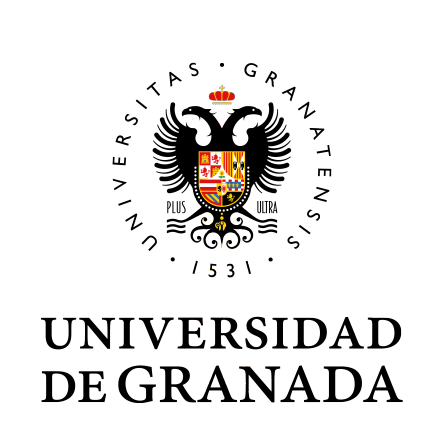
\includegraphics[scale=0.5]{img/ugr.png}\\

\textsc{\Large \asignatura{}\\[0.2cm]}
\textsc{GRADO EN INGENIERÍA INFORMÁTICA}\\[1cm]

\noindent\rule[-1ex]{\textwidth}{1pt}\\[1.5ex]
\textsc{{\Huge \titulo\\[0.5ex]}}
\textsc{{\Large \subtitulo\\}}
\noindent\rule[-1ex]{\textwidth}{2pt}\\[3.5ex]

\end{minipage}

\vspace{0.5cm}

\begin{minipage}{\textwidth}

\centering

\textbf{Autor}\\ {\autor{}}\\[2.5ex]
\textbf{Rama}\\ {Computación y Sistemas Inteligentes}\\[2.5ex]
\vspace{0.3cm}


\includegraphics[scale=0.3]{img/etsiit.jpeg}

\vspace{0.7cm}
\textsc{Escuela Técnica Superior de Ingenierías Informática y de Telecomunicación}\\
\vspace{1cm}
\textsc{Curso 2019-2020}
\end{minipage}
\end{titlepage}

\pagenumbering{arabic}
\tableofcontents
\thispagestyle{empty}				% No usar estilo en la pagina de indice

\newpage

\setlength{\parskip}{1em}

\nonumsection{Ejercicio 1}

\question{Identifique las semejanzas y diferencias entre los problemas
de: a) clasificación de imágenes; b) detección de objetos: c)
segmentación de imágenes; d) segmentación de instancias.}

\answer

\nonumsection{Ejercicio 2}

\question{¿Cuál es la técnica de búsqueda estándar para la detección de
objetos en una imagen? Identifique pros y contras de la misma e
indique posibles soluciones para estos últimos.}

\answer

\nonumsection{Ejercicio 3}

\question{Considere la aproximación que extrae una serie de
características en cada píxel de la imagen para decidir si hay
contorno o no. Diga si existe algún paralelismo entre la forma de
actuar de esta técnica y el algoritmo de Canny. En caso positivo
identifique cuales son los elementos comunes y en que se diferencian
los distintos.}

\answer

\nonumsection{Ejercicio 4}

\question{Tanto el descriptor de SIFT como HOG usan el mismo tipo de
información de la imagen pero en contextos distintos. Diga en que se
parecen y en que son distintos estos descriptores. Explique para que
es útil cada uno de ellos.}

\answer

\nonumsection{Ejercicio 5}

\question{Observando el funcionamiento global de una CNN, identifique que
dos procesos fundamentales definen lo que se realiza en un pase hacia
delante de una imagen por la red. Asocie las capas que conozca a cada
uno de ellos.}

\answer

El primer proceso fundamental es la \textbf{extracción de características}.
Mediante este proceso se puede extraer información relevante sobre la imagen
de entrada. En este proceso intervienen toda una serie de capas,
como las capas convolucionales, las cuáles realizan transformaciones sobre
la imagen de entrada; las capas de activación, las cuáles
introducen alguna función no lineal sobre las salidas de las
capas convoluciones, como por ejemplo la función \texttt{ReLU}; y las
capas de \textit{pooling}, las cuáles realizan una reducción o aumento
del tamaño de la imagen. También se pueden utilizar otras capas en este
proceso las cuáles sirven para regularizar el modelo, como por ejemplo las capas
de \texttt{Dropout} o de \texttt{Batch Normalization}. De esta forma, se puede
llegar a evitar el sobreajuste que se pueda producir en el modelo.

El segundo proceso funtamental es la \textbf{predicción}, la cuál utiliza
la información extraída en el proceso anterior para proporcionar algún tipo
de información de salida. Por ejemplo, se puede predecir a qué clase pertenece una
imagen dada. En esta parte se utilizan normalmente capas totalmente
conectadas con una función de activación determinada en la última capa. En el
ejemplo de clasificación anterior se utilizaría la función \texttt{softmax},
la cuál da un vector de probabilidades para cada una de las clases.

\nonumsection{Ejercicio 6}

\question{Se ha visto que el aumento de la profundidad de una CNN es un
factor muy relevante para la extracción de características en
problemas complejos, sin embargo este enfoque añade nuevos problemas.
Identifique cuales son y qué soluciones conoce para superarlos.}

\answer

Al aumentar la profundidad de la red, se pueden extraer mejores características
de la imagen, y por ende, se pueden aprender funciones más complejas. Sin
embargo, existe un problema con este enfoque, y es que llega un punto en el
que la función que se aprende se empieza a pegar demasiado a los datos
de entrenamiento, y por tanto se produce sobreajuste. Para evitarlo, se pueden
introducir capas de regularización, como por ejemplo \texttt{Batch Normalization},
\texttt{Dropout} o haciendo un \textit{early-stopping}, de forma que
se pare de entrenar antes de que se produzca sobreajuste.

Otro problema que nos encontramos al aumentar la profundidad es que llega un
punto en el que el error propagado por el algoritmo de \texttt{Back Propagation}
es 0, con lo cuál no llega nada a las primeras capas y no se produce un ajuste
de los pesos en función del gradiente. Este problema tiene distintas soluciones,
como por ejemplo modificar la red de forma
la arquitectura no sea secuencial, haciendo que una capa no esté conectada
solamente con la siguiente, si no con otras, como por ejemplo se hace
en la red residual \texttt{ResNet} \cite{DBLP:journals/corr/HeZRS15};
o también introduciendo más de un clasificador en la red, como por ejemplo
en \texttt{GoogLeNet} \cite{DBLP:journals/corr/SzegedyLJSRAEVR14},
de forma que el gradiente no pierda su intensidad.


\nonumsection{Ejercicio 7}

\question{Existe actualmente alternativas de interés al aumento de la
profundidad para el diseño de CNN. En caso afirmativo diga cuál/es y
como son.}

\answer

\nonumsection{Ejercicio 8}

\question{Considere una aproximación clásica al reconocimiento de escenas
en donde extraemos de la imagen un vector de características y lo
usamos para decidir la clase de cada imagen. Compare este
procedimiento con el uso de una CNN para el mismo problema. ¿Hay
conexión entre ambas aproximaciones? En caso afirmativo indique en
que parecen y en que son distintas.}

\answer

\nonumsection{Ejercicio 9}

\question{¿Cómo evoluciona el campo receptivo de las neuronas de una CNN
con la profundidad de la capas? ¿Se solapan los campos receptivos de
las distintas neuronas de una misma profundidad? ¿Es este hecho algo
positivo o negativo de cara a un mejor funcionamiento?}



\answer

\nonumsection{Ejercicio 10}

\question{¿Qué operación es central en el proceso de aprendizaje y
optmización de una CNN?}

\answer

\nonumsection{Ejercicio 11}

\question{Compare los modelos de detección de objetos basados en
aproximaciones clásicas y los basados en CNN y diga que dos procesos
comunes a ambos aproximaciones han sido muy mejorados en los modelos
CNN. Indique cómo.}

\answer

\nonumsection{Ejercicio 12}

\question{Es posible construir arquitecturas CNN que sean independientes
de las dimensiones de la imagen de entrada. En caso afirmativo diga
cómo hacerlo y cómo interpretar la salida.}

\answer

\nonumsection{Ejercicio 13}

\question{Suponga que entrenamos una arquitectura Lenet-5 para clasificar
imágenes $128 \times 128$ de 5 clases distintas. Diga que cambios deberían de
hacerse en la arquitectura del modelo para que se capaz de detectar
las zonas de la imagen donde aparecen alguno de los objetos con los
que fue entrenada.}

\answer

\nonumsection{Ejercicio 14}

\question{Argumente por qué la transformación de un tensor de dimensiones
$128 \times 32 \times 32$ en otro de dimensiones $256 \times 16 \times 16$,
usando una convolución $3 \times 3$ con stride=2, tiene sentido que pueda
ser aproximada por una secuencia de tres convoluciones: convolución $1 \times 1$
+ convolución $3 \times 3$ + convoluión $1 \times 1$. Diga también qué papel
juegan cada una de las tres convoluciones.}

\answer

Esta transformación tiene sentido ya que las convoluciones $1 \times 1$ sirven
para aumentar/reducir la profundidad sin modificar las otras dimensiones del tensor,
mientras que la convolución $3 \times 3$ del segundo modelo va a hacer exactamente
lo mismo que la del modelo original: extraer característsticas y reducir la anchura y
la altura del tensor a la mitad, ya que en ambos casos se utiliza un \texttt{stride = 2}.
Por tanto, lo único nuevo que se introduce en la segunda transformación es la
reducción y el aumento de la profundidad del tensor, conservando convolución central
(la $3 \times 3$). Este segundo enfoque, aunque en un principio parezca que no,
tiene una serie de beneficios.

Por una parte, se consigue un \textbf{aumento de velocidad} ya que el número de operaciones
a realizar es menor. Para ello, siguiendo la línea de lo dicho anteriormente,
la primera convolución $1 \times 1$ reduciría la profundidad del tensor, compactándolo.
La segunda convolución, una $3 \times 3$ con \texttt{stride = 2} se aplicía sobre el
resultado anterior, reduciendo por tanto la anchura y la altura del tensor a la mitad,
pero conservando la profundiad, y extrayendo características en el proceso. Finalmente,
la tercera convolución $1 \times 1$ aumentaría la profundidad del tensor a 256, el tamaño
de salida. De esta forma, tendríamos una arquitectura que consiste
en reducir la dimensionalidad, extraer características y aumentar la dimensionalidad.

Para verlo más claro, vamos a ver las operaciones que se realizan en cada caso
de forma gráfica. Vamos a suponer que en el segundo caso, al reducir la dimensionalidad
con la primera convolución $1 \times 1$ se pasa a 64 canales, ya que no se especifica
nada sobre el número de canales de salida en el enunciado.

\begin{figure}[H]
  \centering
  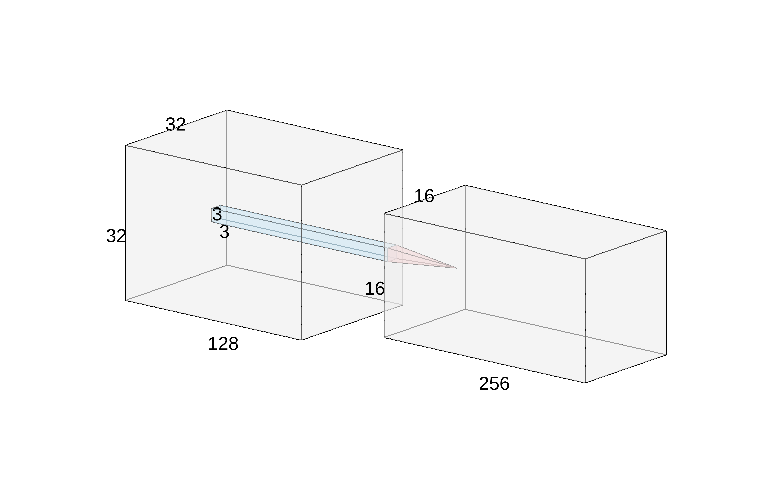
\includegraphics[scale=0.35]{img/cnn1.png}
  \caption{Transformación utilizando una convolución $3 \times 3$ con \texttt{stride = 2}.}
  \label{fig:cnn1}
\end{figure}

\begin{figure}[H]
  \centering
  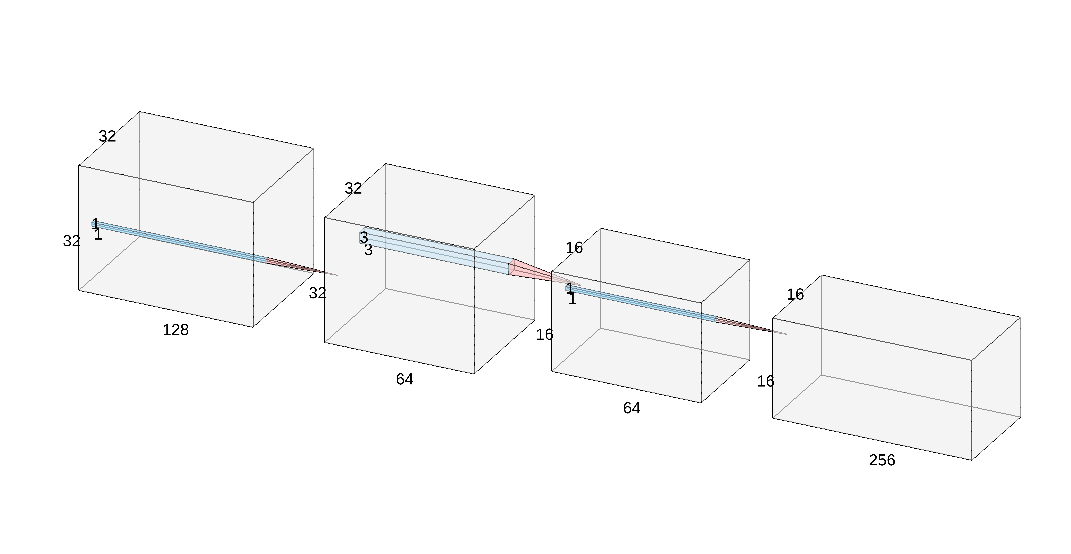
\includegraphics[scale=0.3]{img/cnn2.png}
  \caption{Transformación utilizando tres convoluciones.}
  \label{fig:cnn2}
\end{figure}

Se puede ver que al final el tensor de salida es el mismo, solo que en un
caso se realizan más tranformaciones. Sin embargo, si nos
paramos a analizar el número de operaciones para cada caso, se obtienen
los siguientes resultados:

\begin{itemize}
  \item Para el caso en el que solo se hace una convolución, se hacen
  $128 \times 256 \times 3 \times 3$ operaciones, lo que son unas
  \texttt{295K} operaciones en total aproximadamente.
  \item Para el caso en el que se hacen 3 convoluciones, tenemos que
  en la primera convolución se hacen $128 \times 64 \times 1 \times 1$ operaciones,
  en la segunda $64 \times 64 \times 3 \times 3$ y en la tercera se hacen
  $64 \times 256 \times 1 \time 1$. Este número de operaciones on
  \texttt{8K}, \texttt{36K} y \texttt{16K} operaciones en cada caso,
  lo cuál son en total aproximadamente unas \texttt{60K} operaciones.
\end{itemize}


Por tanto, vemos que en el segundo caso se hacen menos operaciones, y por
consiguiente, será una arquitectura más rápida que la del primer caso.

Por otra, se consigue un \textbf{aumento de la no linealidad}. Esto se debe
a que entre cada capa de convolución se puede insertar una función de activación,
la cuál introduce no linealidad. Este aumento es beneficioso, ya que
se puede conseguir una mejor aproximación a la función real que se quiere aprender,
la cuál es muy difícil que sea lineal (una función lineal es demasiado simple
como para aprender algo así con una red convolucional, para eso podríamos
resolver el problema con un clasificador lineal). En el segundo caso, podemos
introducir hasta tres capas de activación (las cuáles introducen la no linealidad),
mientras que en la primera solo tenemos una activación al final del proceso,
con lo cuál se consigue una aproximación ``peor'' (que no tiene por qué ser mala)
de la función real. Sin embargo, es esta no linealidad la que hace que los
resultados no sean exactamente los mismos en los dos casos, si no que sean aproximados.

 
\nonumsection{Ejercicio 15}

\question{Identifique una propiedad técnica de los modelos CNN que permite
pensar que podrían llegar a aproximar con precisión las
características del modelo de visión humano, y que sin ella eso no
sería posible. Explique bien su argumento.}

\answer

\newpage

\bibliographystyle{plain}
\bibliography{mybib}

\end{document}

